\documentclass[12pt]{article}
%%%%%%%%%%%%%%%%%%%%%%%%%%%%%%%%%%%%%%%%%%%%%%%%%%%%%%%%%%%%%%%%%%%%%%%%%%%%%%%%%%%%%%%%%%%%%%%%%%%%%%%%%%%%%%%%%%%%%%%%%%%%%%%%%%%%%%%%%%%%%%%%%%%%%%%%%%%%%%%%%%%%%%%%%%%%%%%%%%%%%%%%%%%%%%%%%%%%%%%%%%%%%%%%%%%%%%%%%%%%%%%%%%%%%%%%%%%%%%%%%%%%%%%%%%%%
\usepackage{amsfonts}
\usepackage{eurosym}
\usepackage{geometry}
\usepackage{amsmath,amsthm,amssymb}
\usepackage{ulem} 
\usepackage{graphicx}
\usepackage{comment}
%\usepackage[sort,comma]{natbib}
\usepackage[utf8]{inputenc}
\usepackage{setspace}
\usepackage[backend=biber, style = apa]{biblatex}
\usepackage{placeins} % to separate sections

\usepackage{adjustbox}
\usepackage{array}
\usepackage{multirow}
\usepackage{graphicx}
\usepackage{subcaption}
\usepackage{pifont}
\usepackage{amssymb}
\usepackage{comment}
\usepackage[hang, flushmargin, bottom]{footmisc}
\usepackage{footnotebackref}
\usepackage{xcolor}
\usepackage{hyperref}
\usepackage{booktabs}
\usepackage{pifont}
\usepackage{caption}
\usepackage{float}
\usepackage{todonotes}
\setcounter{MaxMatrixCols}{10}


%\setlength{\bibsep}{0.3pt}
\setlength{\textfloatsep}{5pt}
\hypersetup{breaklinks=true,hypertexnames=false,colorlinks=true,citecolor = teal}
\captionsetup{font=normalsize}
\newcommand{\cmark}{\ding{51}}
\def\sym#1{\ifmmode^{#1}\else\(^{#1}\)\fi}
\renewcommand{\thetable}{\Roman{table}}
\geometry{verbose,tmargin=.9in,bmargin=1in,lmargin=.8in,rmargin=.8in,nomarginpar}
\makeatletter
\DeclareTextSymbolDefault{\textquotedbl}{T1}
\theoremstyle{plain}
\newtheorem{thm}{\protect\theoremname}
\theoremstyle{plain}
\newtheorem{prop}[thm]{\protect\propositionname}
\theoremstyle{definition}  % Add this line
\newtheorem{definition}[thm]{Definition}  % Add this line
\theoremstyle{remark}  % Add this line
\newtheorem{remark}[thm]{Remark}  % Add this line
\providecommand{\propositionname}{Proposition}
\newtheorem{proposition}{Proposition}

\providecommand{\theoremname}{Theorem}
\makeatother
\newtheorem{ass}[thm]{Assumption}
% \input{tcilatex}
\usepackage{tikz}
\usetikzlibrary{shapes.geometric, arrows, positioning}


\addbibresource{references.bib}
\begin{document}
This document is to adress modeling questions that Phil raised. 

\subsection*{Moral hazard}
Phil raised the question of moral hazard. He said that the default probability should depend on the interest rate being paid. 

\textbf{\textcite{nelson_private_2025}}

\textcite[1383]{nelson_private_2025} assumes that "borrower default rates depend only on types, and in particular do not depend on prices" which he calls the \textit{price-invariance of default} assumption. He defends the assumption by saying that: 
\begin{itemize}
    \item "First, there is direct evidence that price changes have little to no effect on default rates" to defend this claim he does two things. The first one is that he uses exogenous price variation (a credit card firm repricing their whole portfolio) to "show that the effect of a 100 basis point increase in interest rates on default rates is statistically indistinguishable from zero, and I can reject resultant increases in default rates of more than 0.04 percentage points" moreover he cites \textcite{}
    


    \item " the effect of a change in credit card pricing on a typical consumer’s overall debt service is arguably negligible, suggesting that changes in credit card pricing  8Using the same price variation highlighted below in Section 4.2.2, Appendix Section A.7 shows that the effect of a 100 basis point increase in interest rates on default rates is statistically indistinguishable from zero, and I can reject resultant increases in default rates of more than 0.04 percentage points. This null result is supported by similar findings in the randomized controlled trial of Castellanos, Hernández, Mahajan, and Seira (2025). are unlikely to affect solvency;9
\end{itemize}









\newpage




















\section*{Model 5: Structural Model of Cross-Selling with Asymmetric Information}

This document presents the full structural model. Section~\ref{sec:game} describes the two-stage game and the backward induction approach. Sections~\ref{sec:model}--\ref{sec:bank2profits} solve stage~2 and derive the equilibrium. Section~\ref{sec:stage1} uses the stage~2 solution to characterize stage~1 pricing via backward induction.


%===========================================================================
%  SECTION 1: TWO-STAGE GAME
%===========================================================================

\section{The Two-Stage Game}\label{sec:game}

We model a banking duopoly in which two banks compete for consumers across two sequential product markets. The timing generates both the information asymmetry and the switching costs that are the primitives of the second-stage pricing game.

\begin{center}
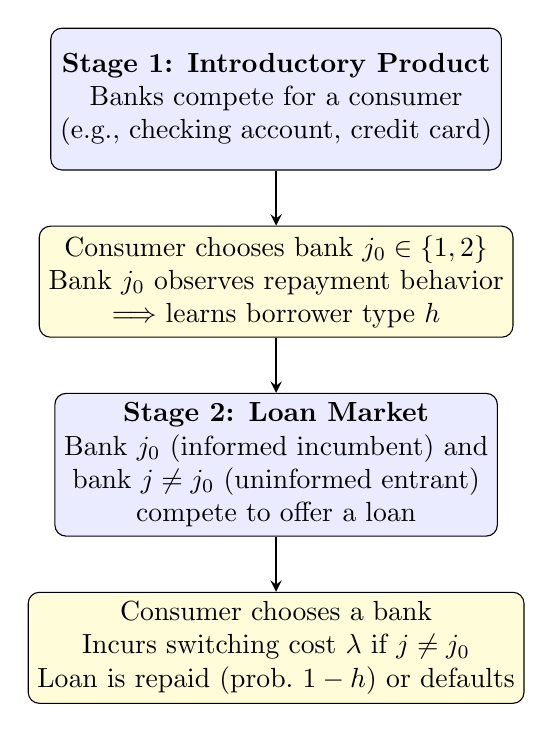
\begin{tikzpicture}[
    stage/.style={rectangle, draw, rounded corners, minimum width=5.5cm, minimum height=1.8cm, align=center, fill=blue!8},
    outcome/.style={rectangle, draw, rounded corners, minimum width=5.5cm, minimum height=1.2cm, align=center, fill=yellow!15},
    arrow/.style={->, thick, >=stealth}
]
\node[stage] (s1) {\textbf{Stage 1: Introductory Product}\\ Banks compete for a consumer\\(e.g., checking account, credit card)};
\node[outcome, below=0.7cm of s1] (o1) {Consumer chooses bank $j_0 \in \{1,2\}$\\Bank $j_0$ observes repayment behavior\\$\Longrightarrow$ learns borrower type $h$};
\node[stage, below=0.7cm of o1] (s2) {\textbf{Stage 2: Loan Market}\\ Bank $j_0$ (informed incumbent) and\\bank $j \neq j_0$ (uninformed entrant)\\compete to offer a loan};
\node[outcome, below=0.7cm of s2] (o2) {Consumer chooses a bank\\Incurs switching cost $\lambda$ if $j \neq j_0$\\Loan is repaid (prob.\ $1-h$) or defaults};

\draw[arrow] (s1) -- (o1);
\draw[arrow] (o1) -- (s2);
\draw[arrow] (s2) -- (o2);
\end{tikzpicture}
\end{center}

\medskip\noindent
\textbf{Stage~1.} Both banks compete to attract a consumer through an \emph{introductory product}---a checking account, a credit card, or a small initial loan. At this stage, neither bank has private information about the consumer's creditworthiness. The consumer chooses one of the two banks (say bank~1). Through the ensuing relationship, bank~1 observes the consumer's repayment history and account behavior, thereby learning the consumer's default probability~$h$.

\medskip\noindent
\textbf{Two consequences of stage~1:}
\begin{enumerate}
    \item \textbf{Information asymmetry.} Bank~1 learns $h$; bank~2 does not. Bank~2 knows only the population distribution of types.
    \item \textbf{Switching costs.} The consumer develops a relationship with bank~1 (e.g., direct deposit, automatic payments, familiar digital platform). Switching to bank~2 for subsequent products imposes a cost $\lambda \geq 0$ on the consumer.
\end{enumerate}

\medskip\noindent
\textbf{Stage~2.} With bank~1 informed and the consumer partially locked in, the two banks compete to offer a loan. This is the \emph{cross-selling} stage: the introductory product was both a financial service in its own right and a mechanism for acquiring the informational advantage that shapes competition in the loan market. The incumbent can price-discriminate across borrower types, while the entrant must set a single rate for all borrowers.

\medskip\noindent
\textbf{Solution approach: backward induction.} We solve the game by backward induction. Sections~\ref{sec:model}--\ref{sec:bank2profits} derive the stage~2 equilibrium, taking as given that one bank has acquired the customer (and hence the information and switching cost advantages). This yields the continuation payoffs for both the incumbent and the entrant. Section~\ref{sec:stage1} then uses these continuation values to characterize stage~1 pricing: each bank's willingness to pay to acquire a customer in stage~1 is pinned down by the stage~2 rents it expects to earn.


%===========================================================================
%  SECTION 2: STAGE 2 MODEL
%===========================================================================

\newpage
\section{Stage 2: Model}\label{sec:model}

There are two banks competing to lend to a consumer who is currently a client of bank~1 (from stage~1). Bank~1 (the \emph{informed/incumbent} bank) observes the borrower's default probability $h$; Bank~2 (the \emph{uninformed/entrant} bank) does not.

\subsection{Demand}

Consumer utility from borrowing from bank $j$ is:
\begin{align*}
    u_{i1} &= -\alpha\, r_{i1} + \varepsilon_{i1} \\
    u_{i2} &= -\alpha\, r_{i2} - \lambda + \varepsilon_{i2}
\end{align*}
where $r_{ij}$ is the interest rate, $\alpha > 0$ governs price sensitivity, $\lambda \geq 0$ is the switching cost incurred when moving to bank~2, and $\varepsilon_{ij}$ capture idiosyncratic preferences. The borrower chooses the bank with higher utility.

We write $s(r_1, r_2)$ for the probability that a borrower chooses the incumbent (bank~1). All results in Sections~\ref{sec:eq}--\ref{sec:properties} hold for any demand function satisfying Assumption~\ref{ass:demand}; Section~\ref{sec:logit} specializes to the logit.

\subsection{Types}

The default probability $h$ is distributed according to CDF $F(h)$ with density $f(h)$ on $[h_{\min}, h_{\max}] \subset (0,1)$, with $f$ bounded away from zero.

\subsection{Strategies}

Bank~1 observes each borrower's type $h$ and sets a type-contingent interest rate:
$$\sigma: [h_{\min}, h_{\max}] \to \mathbb{R}_+, \qquad h \mapsto \sigma(h)$$
Bank~2 does not observe $h$ and sets a single interest rate $r_2 \in \mathbb{R}_+$ for all borrowers.

\subsection{Profit Functions}

A loan to a type-$h$ borrower at rate $r$ yields expected revenue $(1-h)r$ against a unit cost of funds. The per-loan margin is $(1-h)r - 1$ and the break-even rate is $c(h) \equiv \frac{1}{1-h}$.

\medskip\noindent
Bank~1's expected profit from a type-$h$ borrower:
\begin{align}\label{eq:pi1}
    \pi_1(r_1;\, h,\, r_2) = \big[(1-h)\,r_1 - 1\big] \cdot s(r_1, r_2)
\end{align}

\medskip\noindent
Bank~2's expected profit (aggregated over the population):
\begin{align}\label{eq:pi2}
    \pi_2(r_2;\, \sigma) = \int_{h_{\min}}^{h_{\max}} \big[(1-h)\,r_2 - 1\big] \cdot \big[1 - s(\sigma(h), r_2)\big] \, dF(h)
\end{align}

\subsection{Assumptions}

\begin{ass}[Type distribution]\label{ass:F}
$F$ has support $[h_{\min}, h_{\max}] \subset (0,1)$, is absolutely continuous, and its density $f$ is bounded away from zero on $[h_{\min}, h_{\max}]$.
\end{ass}

\begin{ass}[Demand regularity]\label{ass:demand}
The market share function $s: \mathbb{R}_+^2 \to (0,1)$ is $C^2$ and satisfies:
\begin{enumerate}
    \item[(i)] $s_1(r_1, r_2) < 0$ \quad (raising $r_1$ reduces bank~1's share);
    \item[(ii)] $s_2(r_1, r_2) > 0$ \quad (raising $r_2$ increases bank~1's share);
    \item[(iii)] $\ln s(r_1, r_2)$ is strictly concave in $r_1$ for each $r_2$ \quad (log-concavity).
\end{enumerate}
\end{ass}

\begin{ass}[Entrant concavity]\label{ass:pi2conc}
For any measurable $\sigma: [h_{\min}, h_{\max}] \to \mathbb{R}_+$, the aggregate profit $\pi_2(r_2; \sigma)$ is strictly concave in $r_2$. \footnote{\textcolor{red}{here one would need to 1. provide conditions of the primitives such that the profits of the second firm are concave and ideally relax it so that requires quas-concavity.}}
\end{ass}

\begin{remark}
Assumption~\ref{ass:demand}(iii) is equivalent to $s \cdot s_{11} < s_1^2$, i.e., the curvature condition $\frac{d^2}{dr_1^2}\ln s < 0$. Combined with the positive margin at the optimum, it ensures bank~1's profit is strictly quasi-concave in $r_1$, yielding a unique best response for each type. Assumption~\ref{ass:pi2conc} guarantees a unique optimal rate for bank~2. All three assumptions are satisfied by the logit demand (Section~\ref{sec:logit}).
\end{remark}

We define two objects that will appear throughout. The \emph{inverse semi-elasticity} of bank~$j$'s demand is:
\begin{align}\label{eq:markup_def}
    m_1(r_1, r_2) \equiv \frac{s(r_1, r_2)}{-s_1(r_1, r_2)}, \qquad m_2(r_1, r_2) \equiv \frac{1 - s(r_1, r_2)}{s_2(r_1, r_2)}
\end{align}
These are the standard ``markup functions'' from the IO pricing literature: each bank's markup above marginal cost equals $m_j$, as we show next.


%===========================================================================
%  SECTION 3: EQUILIBRIUM
%===========================================================================

\section{Pure Strategy Equilibrium}\label{sec:eq}

\begin{definition}[Pure Strategy Equilibrium]
A pure strategy equilibrium is a pair $(\sigma^*, r_2^*)$ such that:
\begin{enumerate}
    \item For each $h \in [h_{\min}, h_{\max}]$, \; $\sigma^*(h) \in \displaystyle\arg\max_{r_1 \geq 0} \; \pi_1(r_1;\, h,\, r_2^*)$.
    \item $r_2^*  \in \displaystyle\arg\max_{r_2 \geq 0} \; \pi_2(r_2;\, \sigma^*)$.
\end{enumerate}
\end{definition}

\begin{prop}[Equilibrium Characterization]\label{prop:char}
Under Assumptions~\ref{ass:F}--\ref{ass:pi2conc}, any interior pure strategy equilibrium $(\sigma^*, r_2^*)$ is characterized by the following system.

\medskip\noindent
\textbf{(i) Informed bank's pricing rule.} For each $h \in [h_{\min}, h_{\max}]$:
\begin{align}\label{eq:sigma}
    \boxed{\;\sigma^*(h) = \underbrace{\frac{1}{1-h}\vphantom{\Big|}}_{\text{break-even}} + \underbrace{m_1\!\big(\sigma^*(h),\, r_2^*\big)\vphantom{\Big|}}_{\text{markup}}\;}
\end{align}

\medskip\noindent
\textbf{(ii) Uninformed bank's pricing rule.} The rate $r_2^*$ satisfies:
\begin{align}\label{eq:r2foc}
    \int_{h_{\min}}^{h_{\max}} \left[(1-h)\big(1 - s(\sigma^*(h), r_2^*)\big) \;-\; s_2(\sigma^*(h), r_2^*)\, \big((1-h)\,r_2^* - 1\big)\right] dF(h) = 0
\end{align}
Equivalently:
\begin{align}\label{eq:r2star}
    \boxed{\;r_2^* = \frac{1}{1 - \hat{h}} + E_w\!\big[m_2\big]\;}
\end{align}
where $\hat{h} \equiv \frac{\int h\, s_2\, dF}{\int s_2\, dF}$ is the $s_2$-weighted average default probability, $E_w[m_2] \equiv \frac{\int m_2\, s_2\,(1-h)\, dF}{\int s_2\,(1-h)\, dF}$ is the weighted-average markup with weights $w(h) \propto s_2(\sigma^*(h), r_2^*)\,(1-h)\,f(h)$, and all functions are evaluated at $(\sigma^*(h), r_2^*)$.
\end{prop}

\begin{proof}
\textbf{Bank~1's first-order condition.} For each $h$, differentiate \eqref{eq:pi1} with respect to $r_1$:
\begin{align*}
    \frac{\partial \pi_1}{\partial r_1} = (1-h) \cdot s(r_1, r_2) + \big[(1-h)\,r_1 - 1\big] \cdot s_1(r_1, r_2) = 0
\end{align*}
Dividing by $s > 0$ and rearranging:
\begin{align*}
    (1-h) + \big[(1-h)\,r_1 - 1\big] \cdot \frac{s_1}{s} = 0 \qquad\Longrightarrow\qquad (1-h)\,r_1 - 1 = \frac{(1-h)\, s}{-s_1} = (1-h)\, m_1
\end{align*}
which yields \eqref{eq:sigma}. The second-order condition holds: by Assumption~\ref{ass:demand}(iii), $\ln s$ is strictly concave in $r_1$, so $s$ is log-concave; the product of the non-negative linear margin $(1-h)r_1 - 1$ and the log-concave share $s$ is strictly quasi-concave on the relevant domain, ensuring a unique maximizer.\footnote{At $r_1 = c(h) = \frac{1}{1-h}$ the margin is zero; the optimum lies strictly above this.}

\medskip\noindent
\textbf{Bank~2's first-order condition.} Differentiate \eqref{eq:pi2} with respect to $r_2$:
\begin{align*}
    \frac{d\pi_2}{dr_2} = \int_{h_{\min}}^{h_{\max}} \bigg[\underbrace{(1-h)\big(1-s\big)}_{\text{margin effect}} \;+\; \underbrace{\big[(1-h)\,r_2 - 1\big]\cdot(-s_2)}_{\text{share effect}}\bigg] dF(h) = 0
\end{align*}
using $\frac{\partial(1-s)}{\partial r_2} = -s_2$ (raising $r_2$ reduces bank~2's share). This is \eqref{eq:r2foc}.

\medskip\noindent
For the decomposition \eqref{eq:r2star}, rewrite \eqref{eq:r2foc} as:
\begin{align*}
    \int (1-h)(1-s)\, dF = \int s_2 \big[(1-h)\,r_2^* - 1\big]\, dF
\end{align*}
The left side equals $\int m_2 \cdot s_2 \,(1-h)\, dF$ (substituting $1-s = m_2 \cdot s_2$). Expanding the right side:
\begin{align*}
    r_2^* \int s_2(1-h)\, dF - \int s_2\, dF = \int m_2\, s_2\,(1-h)\, dF
\end{align*}
Hence:
\begin{align*}
    r_2^* = \frac{\int s_2\, dF}{\int s_2(1-h)\, dF} + \frac{\int m_2\, s_2\,(1-h)\, dF}{\int s_2\,(1-h)\, dF} = \frac{1}{1 - \hat{h}} + E_w[m_2] \qedhere
\end{align*}
\end{proof}

\begin{remark}[Parallel structure of pricing rules]\label{rem:parallel}
Both banks price at break-even plus a markup, but the nature of the markup differs:
\begin{itemize}
    \item Bank~1 prices \emph{type by type}: for each $h$, it sets break-even $c(h) = \frac{1}{1-h}$ plus the type-specific inverse semi-elasticity $m_1(\sigma^*(h), r_2^*)$.
    \item Bank~2 cannot condition on $h$. It prices at the break-even rate for an ``effective default probability'' $\hat{h}$, plus a \emph{weighted average} of the type-specific markups $m_2(\sigma^*(h), r_2^*)$. The weights $w(h) \propto s_2 \cdot (1-h) \cdot f(h)$ emphasize types for which (a)~bank~2's demand is most price-sensitive (high $s_2$) and (b)~repayment probability is high (low $h$).
\end{itemize}
Both \eqref{eq:sigma} and \eqref{eq:r2star} are implicit equations: the markup on the right-hand side depends on the equilibrium rates.
\end{remark}


%===========================================================================
%  SECTION 4: PROPERTIES
%===========================================================================

\section{Properties of the Equilibrium}\label{sec:properties}

\begin{prop}[Monotone pricing]\label{prop:mono}
Under Assumptions~\ref{ass:F}--\ref{ass:demand}, in any interior equilibrium $\sigma^*(h)$ is strictly increasing in $h$:
\begin{align}\label{eq:dsigma}
    \frac{d\sigma^*}{dh} = \frac{c'(h)}{1 - m_1'(\sigma^*(h), r_2^*)} > 0
\end{align}
where $c'(h) = \frac{1}{(1-h)^2} > 0$ and $m_1' \equiv \frac{\partial m_1}{\partial r_1}$.

Moreover, $m_1' \leq 0$ under log-concavity (Assumption~\ref{ass:demand}(iii)), so $1 - m_1' \geq 1$ and:
\begin{align}\label{eq:dsigma_bound}
    0 < \frac{d\sigma^*}{dh} \leq c'(h) = \frac{1}{(1-h)^2}
\end{align}
with strict inequality when log-concavity is strict. That is, the equilibrium rate increases \emph{more slowly} than the break-even rate, so the markup $m_1(\sigma^*(h), r_2^*)$ is decreasing in $h$.
\end{prop}

\begin{proof}
The equilibrium condition \eqref{eq:sigma} is $\sigma^*(h) = c(h) + m_1(\sigma^*(h), r_2^*)$. Differentiating both sides with respect to $h$ (treating $r_2^*$ as fixed):
\begin{align*}
    \frac{d\sigma^*}{dh} = c'(h) + m_1'\, \frac{d\sigma^*}{dh}
\end{align*}
Solving: $\frac{d\sigma^*}{dh} = \frac{c'(h)}{1 - m_1'}$, which is \eqref{eq:dsigma}.

\medskip\noindent
\emph{Sign of $m_1'$.} Computing $m_1' = \frac{\partial}{\partial r_1}\!\left(\frac{s}{-s_1}\right)$:
\begin{align*}
    m_1' = \frac{s_1(-s_1) - s(-s_{11})}{(-s_1)^2} = \frac{-s_1^2 + s\, s_{11}}{s_1^2} = -1 + \frac{s\, s_{11}}{s_1^2}
\end{align*}
Log-concavity of $s$ states $\frac{d^2}{dr_1^2}\ln s = \frac{s\, s_{11} - s_1^2}{s^2} \leq 0$, hence $s\, s_{11} \leq s_1^2$ and $m_1' \leq 0$. Under strict log-concavity, $m_1' < 0$ strictly, giving the strict bound in \eqref{eq:dsigma_bound}.
\end{proof}

\begin{remark}[Intuition for declining markups]\label{rem:intuition_mono}
The markup $m_1(\sigma^*(h), r_2^*)$ falls with $h$ because riskier borrowers are more contested. As $h$ rises, bank~1 charges a higher rate, pushing borrowers toward bank~2. The resulting competitive pressure compresses bank~1's markup even as the break-even rate rises. This is a general feature: it holds for \emph{any} demand system satisfying Assumption~\ref{ass:demand}, not just the logit.
\end{remark}


\begin{prop}[Adverse selection / Cream-skimming]\label{prop:adverse}
Under Assumptions~\ref{ass:F}--\ref{ass:demand}, in any interior equilibrium, the informed bank cream-skims safe borrowers while the uninformed bank faces an adversely selected pool. Define the demand-weighted average default probabilities:
\begin{align*}
    \bar{h}_1 \equiv \frac{\displaystyle\int h \cdot s(\sigma^*(h), r_2^*)\, dF(h)}{\displaystyle\int s(\sigma^*(h), r_2^*)\, dF(h)}, \qquad
    \bar{h}_2 \equiv \frac{\displaystyle\int h \cdot \big(1-s(\sigma^*(h), r_2^*)\big)\, dF(h)}{\displaystyle\int \big(1-s(\sigma^*(h), r_2^*)\big)\, dF(h)}
\end{align*}
Then:
\begin{align}\label{eq:adverse}
    \bar{h}_1 < E_F[h] < \bar{h}_2
\end{align}
\end{prop}

\begin{proof}
By Proposition~\ref{prop:mono}, $\sigma^*(h)$ is strictly increasing. Since $s_1 < 0$:
\begin{align*}
    \frac{d}{dh}\,s(\sigma^*(h), r_2^*) = s_1 \cdot \frac{d\sigma^*}{dh} < 0
\end{align*}
so $h \mapsto s(\sigma^*(h), r_2^*)$ is strictly decreasing. By Chebyshev's integral inequality applied to the increasing function $h \mapsto h$ and the decreasing function $h \mapsto s(\sigma^*(h), r_2^*)$:
\begin{align*}
    \text{Cov}_F\!\big(h,\; s(\sigma^*(h), r_2^*)\big) < 0 \qquad\Longrightarrow\qquad \bar{h}_1 < E_F[h]
\end{align*}
Similarly, $h \mapsto 1-s(\sigma^*(h), r_2^*)$ is strictly increasing, so $\text{Cov}_F(h,\, 1-s) > 0$, yielding $\bar{h}_2 > E_F[h]$.
\end{proof}

\begin{remark}[Winner's curse interpretation]\label{rem:winners_curse}
The result holds for \emph{any} demand system satisfying Assumption~\ref{ass:demand}: the only input is that $s$ is decreasing in bank~1's rate (which makes $s$ decreasing in $h$ via monotone pricing). The informed bank prices aggressively for safe borrowers and prices high for risky ones, so bank~2 disproportionately attracts borrowers for whom bank~1 chose not to compete---precisely those with high default risk. This is the winner's curse: bank~2 ``wins'' a borrower when bank~1's private information indicates the borrower is a bad bet.
\end{remark}


%===========================================================================
%  SECTION 5: LOGIT SPECIFICATION
%===========================================================================

\section{Logit Specification}\label{sec:logit}

We now specialize the general results to the logit demand arising from i.i.d.\ Type~I extreme value $\varepsilon_{ij}$:
\begin{align}\label{eq:logit_share}
    s(r_1, r_2) = \frac{\exp(-\alpha\, r_1)}{\exp(-\alpha\, r_1) + \exp(-\alpha\, r_2 - \lambda)} = \frac{1}{1 + \exp\!\big(\alpha(r_1 - r_2) - \lambda\big)}
\end{align}
This satisfies Assumptions~\ref{ass:demand} and~\ref{ass:pi2conc}.\footnote{$s_1 = -\alpha\,s(1-s) < 0$; $s_2 = \alpha\,s(1-s) > 0$; $\ln s = -\ln(1+e^{\alpha(r_1-r_2)-\lambda})$ is concave in $r_1$; and aggregate profit log-concavity in $r_2$ follows from Pr\'ekopa's theorem applied to the integrand.}

\subsection{Logit Inverse Semi-Elasticities}

The markup functions \eqref{eq:markup_def} take simple forms:
\begin{align}\label{eq:logit_m}
    m_1 = \frac{s}{-s_1} = \frac{s}{\alpha\, s(1-s)} = \frac{1}{\alpha(1-s)}, \qquad
    m_2 = \frac{1-s}{s_2} = \frac{1-s}{\alpha\, s(1-s)} = \frac{1}{\alpha\, s}
\end{align}

\subsection{Equilibrium Rates}

Substituting into Proposition~\ref{prop:char}:

\medskip\noindent
\textbf{Bank~1 (logit):}
\begin{align}\label{eq:sigma_logit}
    \sigma^*(h) = \frac{1}{1-h} + \frac{1}{\alpha\big(1 - s(\sigma^*(h), r_2^*)\big)}
\end{align}
For given $r_2^*$, this is an implicit equation for $\sigma^*(h)$ for each $h$.

\medskip\noindent
\textbf{Bank~2 (logit):}
\begin{align}\label{eq:r2_logit}
    r_2^* = \frac{1}{1 - \tilde{h}} + \frac{1}{\alpha}\cdot\frac{\displaystyle\int (1-s)(1-h)\, dF}{\displaystyle\int s\,(1-s)(1-h)\, dF}
\end{align}
where $\tilde{h} = \frac{\int h\, s(1-s)\, dF}{\int s(1-s)\, dF}$ and all shares are evaluated at $(\sigma^*(h), r_2^*)$.\footnote{This uses $s_2 = \alpha\,s(1-s)$, so the $s_2$-weights in \eqref{eq:r2star} become $s(1-s)$-weights.} The weights $\propto s(1-s)$ peak at $s = \frac{1}{2}$, emphasizing the most contested borrower types.


%===========================================================================
%  SECTION 6: UNINFORMED BANK PROFITS
%===========================================================================

\section{Uninformed Bank Profits}\label{sec:bank2profits}

In classical models without product differentiation, the uninformed bank earns zero expected profits. With logit demand, this is no longer the case: product differentiation (taste shocks) guarantees bank~2 strictly positive profits, though adverse selection erodes them relative to the symmetric-information benchmark.

\subsection{Strictly Positive Profits}

\begin{prop}[Bank~2 earns strictly positive profits]\label{prop:b2positive}
In any interior equilibrium of the logit model, $\pi_2(r_2^*; \sigma^*) > 0$.
\end{prop}

\begin{proof}
It suffices to exhibit a feasible rate yielding strictly positive profit, since the optimum $r_2^*$ does at least as well.

Set $\hat{r} = \frac{1}{1 - h_{\min}} + \varepsilon$ for some $\varepsilon > 0$. Then for every $h \in [h_{\min}, h_{\max}]$:
\begin{itemize}
    \item The margin $(1-h)\hat{r} - 1 \geq (1-h_{\min})\hat{r} - 1 > 0$ is strictly positive for the safest type and remains non-negative at least on a neighborhood $[h_{\min}, h_{\min} + \delta]$.\footnote{Specifically, $(1-h)\hat{r} > 1$ iff $h < 1 - 1/\hat{r}$, and $1 - 1/\hat{r} > h_{\min}$ by construction.}
    \item The logit share $1 - s(\sigma^*(h), \hat{r}) > 0$ for all $h$, since the logit never assigns zero probability.
\end{itemize}
Therefore the integrand in $\pi_2(\hat{r}; \sigma^*)$ is strictly positive on $[h_{\min}, h_{\min} + \delta]$ and bounded below, so $\pi_2(\hat{r}) > 0$. Since $r_2^*$ is optimal, $\pi_2(r_2^*) \geq \pi_2(\hat{r}) > 0$.
\end{proof}

\begin{remark}[Why classical models give zero profits]
In models without preference heterogeneity, demand is discontinuous: a borrower deterministically chooses the cheapest offer (adjusted for switching costs). The informed bank can always undercut the uninformed bank for profitable types, forcing bank~2 into a mixed strategy that earns zero expected profit (the standard Bertrand logic). Logit demand breaks this mechanism: even when bank~1 undercuts bank~2, some borrowers still choose bank~2 due to taste shocks. This residual demand provides a positive profit floor.
\end{remark}

\subsection{Profit Decomposition}

Bank~2's equilibrium profit can be decomposed by separating profitable from unprofitable borrower types. Define the \emph{break-even type for bank~2}:
\begin{align}\label{eq:hdagger}
    h^\dagger \equiv 1 - \frac{1}{r_2^*}
\end{align}
This is the default probability at which bank~2's per-loan margin $(1-h)r_2^* - 1$ equals zero. Types with $h < h^\dagger$ are profitable for bank~2; types with $h > h^\dagger$ generate losses.

\medskip\noindent
Then:
\begin{align}\label{eq:pi2_decomp}
    \pi_2(r_2^*; \sigma^*) = \underbrace{\int_{h_{\min}}^{h^\dagger} \big[(1-h)\,r_2^* - 1\big]\big(1-s\big)\, dF(h)}_{\displaystyle\pi_2^+ > 0 \;\text{(gains from safe types)}} \;+\; \underbrace{\int_{h^\dagger}^{h_{\max}} \big[(1-h)\,r_2^* - 1\big]\big(1-s\big)\, dF(h)}_{\displaystyle\pi_2^- < 0 \;\text{(losses from risky types)}}
\end{align}

The adverse selection result (Proposition~\ref{prop:adverse}) is directly visible here: bank~2's share $1-s(\sigma^*(h), r_2^*)$ is \emph{increasing} in $h$, so it captures a disproportionately large share of the loss-making risky types ($h > h^\dagger$) and a disproportionately small share of the profitable safe types ($h < h^\dagger$). The losses $\pi_2^-$ are the direct cost of the winner's curse.

\begin{remark}[Adverse selection cost]\label{rem:as_cost}
Define the \emph{adverse selection cost} as the profit gap relative to a hypothetical uninformed bank that faces the unconditional type distribution (i.e., whose share does not covary with $h$):
\begin{align}\label{eq:AS_cost}
    \Delta^{AS} \equiv \underbrace{\bar{s}_2 \int \big[(1-h)\,r_2^* - 1\big]\, dF(h)}_{\text{profit without adverse selection}} \;-\; \underbrace{\pi_2(r_2^*;\sigma^*)}_{\text{actual profit}}
\end{align}
where $\bar{s}_2 = \int (1-s)\, dF$ is bank~2's average market share. The first term computes bank~2's profit if its share were constant at $\bar{s}_2$ across all types (no adverse selection). By Chebyshev's inequality---since $1-s$ is increasing in $h$ and the margin $(1-h)r_2^* - 1$ is decreasing in $h$---the covariance between share and margin is negative, so $\Delta^{AS} > 0$: adverse selection strictly reduces bank~2's profit.
\end{remark}

\subsection{Comparative Statics}

\begin{prop}[Effect of $\alpha$ and $\lambda$ on bank~2 profits]\label{prop:b2compstat}
In the logit equilibrium:
\begin{enumerate}
    \item As $\alpha \to \infty$ (homogeneous preferences), $\pi_2 \to 0$. The model converges to the classical zero-profit result.
    \item As $\alpha \to 0$ (extreme differentiation), bank~2's market share approaches $\frac{1}{2}$ for all types and adverse selection vanishes. Bank~2's profit approaches that of a symmetric duopolist facing the average type.
    \item Higher switching costs $\lambda$ reduce bank~2's profit: they lower $1-s$ for all types, shrinking bank~2's share while amplifying the adverse selection pattern.
\end{enumerate}
\end{prop}

\begin{proof}[Proof sketch]
\emph{(1)} As $\alpha \to \infty$, the logit share converges to a step function: $s \to \mathbf{1}(\sigma^*(h) < r_2^* + \lambda/\alpha)$. For types where bank~1 undercuts, $1-s \to 0$ and bank~2 gets no demand. For types where bank~1 does not undercut, the informed bank has already set a rate above bank~2's (signaling that these are the risky types), so the margin $(1-h)r_2^* - 1$ tends to be negative or small. In the limit, bank~2 only attracts unprofitable borrowers, and $\pi_2 \to 0$.

\emph{(2)} As $\alpha \to 0$, rates become irrelevant for demand ($s \to e^{\lambda}/(1+e^{\lambda})$ for all types). Both banks earn the same margin from each type, there is no cream-skimming, and bank~2's profit converges to $\frac{1}{1+e^{\lambda}} \int [(1-h)r_2^* - 1]\, dF(h)$.

\emph{(3)} Increasing $\lambda$ shifts $s$ upward for all $(r_1, r_2)$ pairs, directly reducing $1-s(\sigma^*(h), r_2^*)$ for every type. This lowers both $\pi_2^+$ and $|\pi_2^-|$ in \eqref{eq:pi2_decomp}, but the effect on $\pi_2^+$ dominates because bank~2 already has low share among safe types where its margin is positive.
\end{proof}

\begin{remark}[What sustains bank~2's profits]
Bank~2's strictly positive profit rests entirely on product differentiation: the taste shocks $\varepsilon_{ij}$ ensure that some borrowers choose bank~2 even when it offers a higher rate than bank~1. These ``captive'' borrowers of bank~2 provide a profit floor that is absent in homogeneous-demand models. The economic content is that even an informationally disadvantaged competitor can survive and profit if borrowers have idiosyncratic preferences---whether due to branch location, service quality, digital platform, or relationship factors not captured by the interest rate.

However, bank~2's profit is bounded above: adverse selection ensures it earns less than it would under symmetric information, and switching costs compound this disadvantage. The uninformed bank is profitable but disadvantaged, with the degree of disadvantage governed by the interaction of $\alpha$ (substitutability) and $\lambda$ (lock-in).
\end{remark}


%===========================================================================
%  SECTION 7: STAGE 1 — BACKWARD INDUCTION
%===========================================================================

\newpage
\section{Stage 1: Backward Induction}\label{sec:stage1}

Having solved the stage~2 equilibrium, we now apply backward induction to characterize stage~1 pricing. Each bank anticipates the stage~2 continuation game and sets its introductory price accordingly.

\subsection{Continuation Values from Stage~2}

The stage~2 equilibrium $(\sigma^*, r_2^*)$ determines each bank's expected profit conditional on its role. Since the game is symmetric ex ante---each bank could end up as the incumbent or the entrant---the relevant objects are the \emph{continuation values} of being the home bank versus the rival bank.

\medskip\noindent
\textbf{Continuation value of the incumbent (home bank).} The bank that acquires the customer in stage~1 becomes the informed incumbent in stage~2 and earns:
\begin{align}\label{eq:V_I}
    V^{I} \;\equiv\; \int_{h_{\min}}^{h_{\max}} \underbrace{\big[(1-h)\,\sigma^*(h) - 1\big]}_{\text{per-loan margin}} \cdot \underbrace{s\!\big(\sigma^*(h),\, r_2^*\big)}_{\text{retention probability}} \; dF(h)
\end{align}
This is the expected stage~2 profit of the informed bank, integrating over the borrower type it will face. $V^I > 0$ since the incumbent earns a positive margin on every type it retains (the markup $m_1 > 0$ ensures $\sigma^*(h) > c(h)$).

\medskip\noindent
\textbf{Continuation value of the entrant (rival bank).} The bank that \emph{does not} acquire the customer in stage~1 becomes the uninformed entrant in stage~2 and earns:
\begin{align}\label{eq:V_E}
    V^{E} \;\equiv\; \pi_2(r_2^*;\, \sigma^*) = \int_{h_{\min}}^{h_{\max}} \big[(1-h)\,r_2^* - 1\big] \cdot \big[1 - s(\sigma^*(h),\, r_2^*)\big] \; dF(h)
\end{align}
By Proposition~\ref{prop:b2positive}, $V^E > 0$ under logit demand, though $V^E < V^I$: the incumbent's informational advantage and the consumer's switching costs make the home position strictly more valuable.\footnote{$V^I > V^E$ follows because the incumbent earns positive margins on all types it retains while optimally targeting each type, whereas the entrant faces adverse selection and prices uniformly.}

\medskip\noindent
\textbf{Net value of acquiring a customer.} The incremental value of being the incumbent rather than the entrant is:
\begin{align}\label{eq:DeltaV}
    \Delta V \;\equiv\; V^I - V^E > 0
\end{align}
This is the maximum amount a bank would be willing to sacrifice in stage~1 to acquire the customer.

\subsection{Stage~1 Pricing Problem}

\fcolorbox{red}{yellow!10}{\parbox{0.95\textwidth}{\color{red}\textbf{TODO:} The first-stage profit function below is not correct. (1) The functional form uses an introductory-product margin $p^{(1)} - c^{(1)}$, but if stage~1 is a loan market the profit should be $E_h[(1-h)\,r_{j1} - 1]$. (2) The choice probability $q(\cdot)$ should use the same demand system $s(\cdot)$ as stage~2 (logit with switching cost set to zero in period~1). These issues need to be fixed before using this section for estimation.}}

\bigskip

In stage~1, both banks simultaneously set prices $p_1^{(1)}$ and $p_2^{(1)}$ for the introductory product.\footnote{We use superscript $(1)$ to denote stage~1 variables and distinguish them from stage~2 rates $r_1, r_2$.} The consumer's stage~1 utility from choosing bank~$j$ is:
\begin{align}\label{eq:u_stage1}
    u_j^{(1)} = v - p_j^{(1)} + \eta_j
\end{align}
where $v$ is the common value of the introductory product and $\eta_j$ captures idiosyncratic preferences (analogous to $\varepsilon_{ij}$ in stage~2). Let $q(p_1^{(1)}, p_2^{(1)})$ denote the probability that the consumer chooses bank~1 in stage~1.

\medskip\noindent
Bank~1's total expected profit across both stages is:
\begin{align}\label{eq:total_profit}
    \Pi_1 \;=\; \underbrace{q\!\left(p_1^{(1)}, p_2^{(1)}\right) \cdot \left[\;\underbrace{\left(p_1^{(1)} - c^{(1)}\right)}_{\text{stage~1 margin}} + \underbrace{V^I}_{\text{continuation as incumbent}}\;\right]}_{\text{win the customer}} \;+\; \underbrace{\left(1 - q\!\left(p_1^{(1)}, p_2^{(1)}\right)\right) \cdot V^E}_{\text{lose the customer}}
\end{align}
where $c^{(1)}$ is the marginal cost of providing the introductory product. Rearranging:
\begin{align}\label{eq:total_profit2}
    \Pi_1 = q \cdot \big[\,p_1^{(1)} - c^{(1)} + \Delta V\,\big] + V^E
\end{align}
Since $V^E$ is a constant (it does not depend on bank~1's stage~1 price), bank~1's stage~1 problem reduces to:
\begin{align}\label{eq:stage1_max}
    \boxed{\;\max_{p_1^{(1)}} \;\; q\!\left(p_1^{(1)}, p_2^{(1)}\right) \cdot \left[\,p_1^{(1)} - \big(c^{(1)} - \Delta V\big)\,\right]\;}
\end{align}
This is a standard pricing problem with \emph{effective marginal cost} $c^{(1)} - \Delta V$. The stage~2 continuation value $\Delta V$ acts as a subsidy: each bank is willing to price the introductory product below cost by up to $\Delta V$ in order to acquire the customer and secure the more valuable incumbent position in stage~2.

\subsection{Implications}

\begin{remark}[Loss-leading]
If $\Delta V > c^{(1)}$, the effective marginal cost is negative, and the equilibrium introductory price $p^{(1)*}$ may be below the actual cost $c^{(1)}$---the bank \emph{loses money} on the introductory product to acquire the customer. This is the \emph{loss-leading} phenomenon: the introductory product is priced as a loss leader because the real profit comes from the cross-sold loan in stage~2.
\end{remark}

\begin{remark}[Welfare]
The consumer benefits from below-cost introductory pricing in stage~1 but pays above-competitive rates in stage~2 (due to the incumbent's information advantage and switching costs). The net welfare effect depends on the magnitude of $\Delta V$ relative to the stage~2 markup. Specifically, as $\lambda$ or the information asymmetry increase, $\Delta V$ rises (more stage~2 rents to compete for), so stage~1 prices fall further. But stage~2 markups also rise. The overall effect on consumer welfare is ambiguous and depends on the estimated structural parameters $(\alpha, \lambda, F)$.
\end{remark}

\begin{remark}[Symmetric equilibrium]
By symmetry---both banks face the same continuation values and the same stage~1 demand structure---the stage~1 equilibrium is symmetric: $p_1^{(1)*} = p_2^{(1)*} = p^{(1)*}$. The equilibrium introductory price satisfies the standard first-order condition with the adjusted marginal cost:
\begin{align}\label{eq:p1_foc}
    p^{(1)*} = \big(c^{(1)} - \Delta V\big) + m^{(1)}(p^{(1)*})
\end{align}
where $m^{(1)}$ is the inverse semi-elasticity of stage~1 demand, analogous to the markup functions in stage~2. Higher stage~2 rents ($\Delta V$) translate directly into lower stage~1 prices.
\end{remark}


\end{document}
